%\section{Related Work}\label{Related}

	室內定位研究大部分是利用訊號接收作三角定位,但是需要設備上的支援,如:紅外線、超聲波、Wifi 等設備,訊號的不穩定也會影響定位的誤差。
之後有研究把影像特徵點當作訊號作定位研究,影像定位可以減少訊號不穩定導致的定位誤差,但是照片取樣分布不均及相機角度上的限制,使得室內定位
可定位的範圍受到很大的限制。我們方法利用照片組建出3D點雲環境,在3D環境內拍攝虛擬相片作定位,彌補訊號不穩定的情形及增加可定位的範圍。在相
關研究的章節中我們分成三個階段來說明使用的研究技術。首先基於現今室內定位的研究作探討,再來說明本文方法中3D環境技術的相關研究,最後說明如
何在照片中找到特徵點及特徵點批倍的方法。

\section{室內定位的相關研究}

	 現在室內定位的技術多用於訊號接收定位,需要設備上的支援,下面介紹幾種常用的技術:

  紅外線技術:紅外線室內定位技術定位的原理是,紅外線IR標識的紅外射線,通過安裝在室內的光學傳感器接收進行定位。雖然紅外線具有相對較高的室內
定位的精準度,但是由於光線不能穿過障礙物,當標識放在口袋裡或者有牆壁及其他遮擋時就不能正常工作。因此,紅外線只適合短距離傳播,而且容易被房間
內的燈光所干擾,在定位上有一定的限制。

  超聲波技術:超聲波測距主要採用反射式測距法,通過三角定位等算法確定物體的位置,即發射超聲波並接收由被測物產生的回波,根據回波與發射波的時
間差計算出待測距離。當同時有3個或3個以上不在同一直線上的應答器做出回應時,可以根據相關計算確定出被測物體所在的二維坐標系下的位置。超聲波定位
整體定位精度較高,結構簡單,但超聲波需要大量的底層硬體設施投資,成本太高。

  藍牙技術:藍牙技術通過測量訊號強度進行定位。這是一種短距離低功耗的無線傳輸技術,在室內安裝適當的藍牙裝置,配置成多用戶的連接模式,並保證
此藍牙設備始是這個區域內的主要設備,就可以獲得用戶的位置訊息。藍牙技術主要應用於小範圍定位,例如大廳或倉庫。藍牙室內定位技術最大的優點是設備
體積小、易於作在PDA、PC以及手機中,因此很容易推廣普及。但不足在於藍牙器材和設備的價格比較昂貴,而且對於復雜的空間環境,藍牙系統的穩定性稍差
,受信號干擾大。

  Wi-Fi技術:無線區域網路(WLAN)是一種訊息平台,可以在廣泛的應用領域內實現複雜的大範圍定位、監測和追踪任務[10],而網路節點自身定位是大多
數應用的基礎和前提。當前比較流行的Wi-Fi定位是IEEE802.11無線網路標準的定位解決方案。易於安裝,只需要很少的Access Point(AP)設備,也能採
用相同的底層無線網絡架構,定位精準度高。但是,如果定位的測算僅僅依賴於哪個AP點最近,而不是依賴合成的訊號強度,那麼在樓層定位上很容易出錯。目
前,它應用於小範圍的室內定位,成本較低。但無論是用於室內還是室外定位,Wi-Fi收發器都只能覆蓋半徑90公尺以內的區域,而且很容易受到其他信號的干
擾,從而影響其精度,定位器的能耗也較高。

  ZigBee技術:ZigBee是一種新興的短距離、低速率無線網絡技術,可以用於室內定位。它有自己的無線電標準,在數千個微小的感測器之間互相傳送訊息
以實現定位。這些感測器只需要很少的能量,以接力的方式通過無線電波將數據從一個感測器傳到另一個感測器,所以它們的傳送效率非常高。ZigBee最顯著的
特點是它的低功耗和低成本。

  除了以上提及的定位技術,還有基於電腦視覺、圖像分析、磁場定位等。圖像分析定位就是我們這次所研究的目標,目的可以減低設備上的使用成本,也包含
更多關於整體環境的資訊。


\section{SLAM 在建置3D環境的應用}

%介紹SLAM起源
	上個章節介紹一些室內定位的方法,接下來的章節將介紹Simultaneous Localization and Mapping(SLAM)的方法,以及相關的研
究。SLAM 是利用拍攝路徑的連串影像,針對這些影像的相對關係來製作出一條可被看見的路徑。由Harris和Pike在1987年所提
\cite{Harris198887}的方法,利用連串的影像拼湊出一個影像路徑的地圖,當初的這項研究為最早SLAM的起源。這方法可以秀出路徑上特定
的3D特徵,但是卻無法找出這些3D特徵點的相對關係。這方法因為特徵點之間沒有相對關係,導致找出的路徑與實際影像路徑有所差異,且所做出的
路徑無法封閉,也就是說根據這條路徑沒辦法走回原點。在之後的方法,找出路徑上特徵點的相對關係以及做出一條封閉的路徑,就成了改進SLAM的
研究目標。

%說明SLAM技術的核心
	在之後的研究,像是\cite{174711}、\cite{1087373}與\cite{Smith1988},都朝找出特徵點對應關係,這個方向做加強。這些研究的
共同點都是以 Extended Kalman Filter(EKF)來做路徑分析,EKF方法主要是說,由現在的狀態去預測出未來會發生的情況,利用最大似然
估算法(Maximum Likelihood)來找出最有可能發生的情況,運用在SLAM上面則是改善了特徵點與特徵點相互對應的情況,藉由特徵點分布找出最
有可能的連通關係,形成一個封閉的路徑。由於科技的進步加快運算的速度,在\cite{Betge1996}與\cite{Davison2001}的研究把EKF 
SLAM技術用在一般室內環境之中,也經實驗證實FKF能有效改善SLAM預估出來的路徑所產生的誤差。這對SLAM研究上有了新的發展方向,也有其他
研究把機率模型應用在SLAM改善路徑誤差,像是\cite{Durrant2003}的研究。

%介紹SLAM用在3D model	的情形
	在現今的研究中,有很多的研究利用SLAM來建置3D模型,SLAM在應用上的好處在於增加影像之間匹配關係,以及可用在一般室內環境中。


\section{特徵點的比對與匹配}

	建置3D模型中,我們的方法利用Graph SLAM方法來減少相片之間匹配的錯誤,在上個章節介紹了SLAM的相關研究後,在這個章節我們將說明
如何利用照片找出特徵點,及特徵點匹配的相關研究。找出圖形特徵點及匹配特徵點,目的在不同的照片中拍攝到相同的景物,利用同樣的景物找出兩
個照片相對應的特徵點,再利用特徵點求出這些相片的的相對位置,決定如何將照片放置在3D環境中。基於這項目的,先利用SIFT找出特徵點,再用
RANSAC找出特徵點匹配的關係,使得照片能夠在正確的位置重合。下面的章節將介紹SIFT與RANSAC的方法。
	
\subsection{SIFT 尺度不變特徵向量}
%SIFT 特徵點描述方法
	取出相片中特徵點的方法,一開始由 lowe \cite{Lowe2004} 所提出,稱為尺度不變特徵向量(SIFT)。後來有人針對SIFT做演算法的加速
(SURF)\cite{Bay2006}以及增強找出特徵點數量的方法(ASIFT)\cite{Guo2009}。SURF的方法雖然快速,但是簡化許多計算流程,影響找出
圖片當中特徵點的數量,如果套用在我們的方法中,會導致之後特徵點無法做到有效的匹配。ASIFT是將照片可能會旋轉、放大或縮小的情況考慮進去
,將這些照片模擬不同變化,再根據不同變化的照片中找出匹配的特徵點。此舉會導致運算量的增加,考慮到龐大的運算量導致時間的增加,我們還是
使用一般的SIFT方法找出特徵點。

	尺度不變特徵向量(SIFT),主要分成四個階段:

 \begin{enumerate}
	  \item 區域空間極值分布	
	  \item 特徵點定位與篩選
	  \item 特徵點方向分配
	  \item 特徵點描述向量建立
 \end{enumerate}

   第一階段(1) 區域空間極值篩選,先利用不同尺度間的高斯金字塔選擇區域中的最大極值,其高斯分布式子如下:
\begin{align}
  G(x,y,\sigma) = \frac{1}{2\pi\sigma^2}exp(-(x^2+y^2)/2\sigma^2) 
\end{align}

	不同尺度的高斯分布利用摺積 (Convolution) 將影像模糊化。 $I(x,y)$代表原始影像,$G(x,y,\sigma)$代表高斯函數:	
\begin{align}
  L(x,y,\sigma) = G(x,y,\sigma)\ast{I(x,y)}
\end{align}

\begin{figure}
  \begin{center}
    \subfigure[高斯差分與影像金字塔]{\label{fig:Gaussian Prymaid}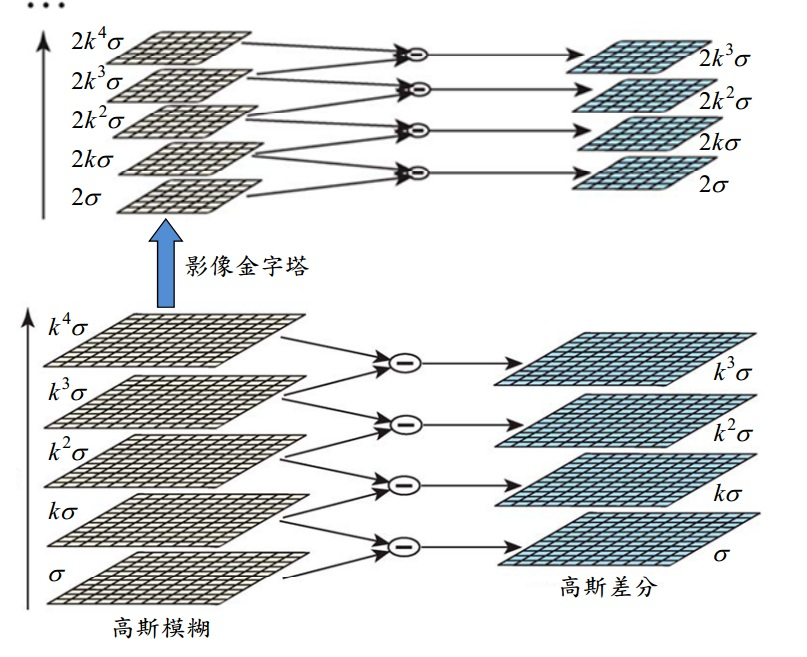
\includegraphics[width=0.45\columnwidth]{figures/Gaussian_Prymaid.jpg}}
    \subfigure[尺度極值偵測]{\label{fig:Extreme Value Detect}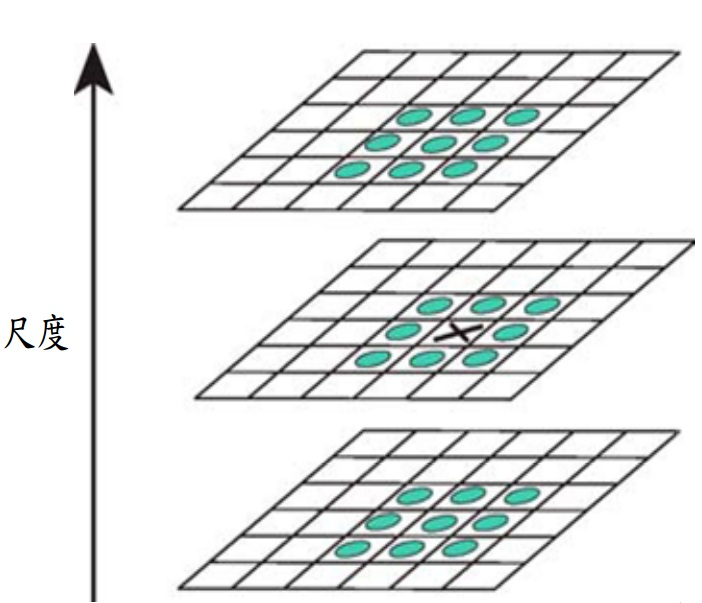
\includegraphics[width=0.45\columnwidth]{figures/extreme_value_detect.jpg}}
  \end{center}
  \caption{glFrustrum 矩陣圖示說明}
  \label{fig:SIFT_explanation}
\end{figure}

  再利用每組影像相鄰的高絲模糊影像進行高斯差分(Difference-Of-Gaussian),目的用於在集合內4組高斯差分影像中找出極值
  ,式子如(1.3)所示:    
\begin{align}
  D(x,y,\sigma) = L(x,y,k\sigma)-L(x,y,\sigma)
\end{align}

  在此k為高斯模糊的尺度比值,設為$\sqrt{2}$,若某個像素的極值為26個相鄰的像素中最大或最小的話,則此像素的位址即為區域極值的所在。

  第二階段(2) 特徵點定位篩選,其主要的目的在於找出真正有用的特徵點,在此特徵點的精準度必須要達到次像素的精度。有的特徵點其極值為低對比度的點,這時候這些低對比度的特徵點就會不予採用,剩下的特徵點即可為
下一階段所使用。作法首先將(1.3)利用泰勒展開得到(1.4): 
\begin{align}
  D(x) = D + \frac{\delta D^T}{\delta X}X + \frac{1}{2}X^T\frac{\delta^2 D}{\delta X^2}X
\end{align}

   式中$X$為極值$(x,y,\delta)^T$,$D$為高斯差分後的結果,再將(1.4)對$X$作偏微分可得$\vec{X}$算出$X$為極值點的的偏移量。
   
\begin{align}
  \vec{X} = -\frac{\delta^2 D}{\delta X^2}^{-1}\frac{\delta D}{\delta X}
\end{align}   
   
   
   若是$\vec{X} >= 0.5$,或是 $\sigma > k/2$,表示此區域極值點較靠近相鄰的點位,則需要再將此點移至相鄰的極值再經(1.5)計算後得到最佳的位置。若將$\vec{X}$帶入(1.4)中,可得(1.6)我們所用來篩選的式子:  
\begin{align}
  D(\vec{X}) = D+\frac{1}{2} \frac{\sigma D^T}{\sigma X} \vec{X}
\end{align}      
   
   利用(1.6)將求出的絕對值與其他絕對值相比,可將對比度小的特徵點刪除以達到過濾的效果。
   
   第三階段(3) 特徵點方向分配,目的在於當對比的圖片有旋轉或者是尺度上的變化,相同的特徵點為了保有相同方向的特性,必須賦予每個特徵點一組特定的方向。其做法則是利用統計的方式,將所有的梯度值以角度每10個單位做方位直方圖記錄,
並且記錄每個梯度的強度,以(1.7)(1.8)表示:
\begin{align}
	\theta (x,y)= tan^{-1}(\frac{\delta L}{\delta y}/\frac{\delta L}{\delta x}))
\end{align}      
   
\begin{align}
	m(x,y) = \sqrt{(\frac{\delta L}{\delta x})^2+(\frac{\delta L}{\delta y})^2}
\end{align}


   第四階段(4)徵點描述向量建立,最後一個階段為提供特徵點作為依據。做法上先將影像旋轉,使其特徵點向量與畫面主方巷一致之後
   ,再以特徵點為中心,作出一個$16 x 16$的視窗,並加一個尺度為$0.5\sigma$的高斯函數為權重。把每個區塊區分成$4 x 4$的大小,
   切割成 16 個區塊,在每個區塊統計出梯度方位$ \theta (x,y)$以及強度值$m(x,y)$,而後分別每個區塊有 8 個區間,代表 8 
   個不同的方向,如 \ref{fig:SIFT Histogram} 所表示。

\begin{figure*}
\begin{center}
  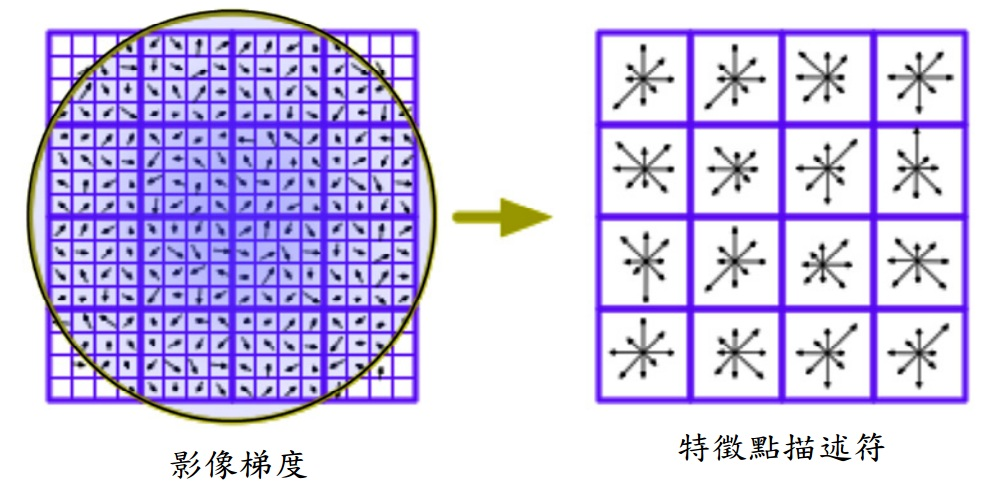
\includegraphics[width=0.8\textwidth]{figures/SIFT_histogram.jpg}
  \caption{特徵點向量方為與強度示意直方圖}
  \label{fig:SIFT Histogram}
\end{center}
\end{figure*}  

     每個特徵點有 16 個方位的直方圖,每個方位直方圖內有 8 個梯度強度值,因此共有$ 16 x 8 = 128$個特徵值,
     這些特徵點則為我們所需要的描述向量。

\subsection{隨機抽樣一致演算法(RANSAC)}

	在獲得照片2D特徵點的資訊後,利用這些照片與Kinect的深度資訊做結合,建置3D環境。但是找出的特徵點當中,包含深度錯誤的資訊,為了將這些錯誤的資訊過濾掉,利用
RANSAC(RANdom Sample Consensus)將不必要的深度特徵刪除,使得作出的轉移矩陣能將3D影像投影至正確的位置。RANSAC\cite{Fischler1981}由1981年被提出,大
多運用在電腦視覺上,用來預測數學模型有可能分布的狀況,透過迭代的方法使得預測的精準度增加。

	RANSAC的流程分為下面幾個步驟:
 \begin{enumerate}
	  \item 設定隨機挑選的inlier數量n,以及迴圈的重複次數k
	  \item 從所有的匹配中隨機挑選n個作為inliers,數量至少能夠計算出轉移矩陣
	  \item 以Levenberg-Marquardt演算法從inliers計算出投影矩陣$R_{in}$
	  \item 把inliner之外的匹配特徵帶入$R_in$,計算投影之後匹配特徵的距離,把距離小於設定門檻值得闢配都加入inliers
	  \item 紀錄所有iinliers,並比較其總數受否大於現在的最大值,如果是則更新最大值
	  \item 重複執行k次步驟2.到步驟5.,最後留下的最大值就是過濾好的特徵點,再利用Levenberg-Marquardt蟲這些過濾好的批被去計算出最佳轉移矩陣$R_{best}$
 \end{enumerate}

	至於n和k如何決定,可以假設每個特徵匹配為良好的機率設w,因此一開始隨機挑選的n個匹配的機率為$W^n$,其中涉某個錯誤的機率為$1-W^n$,而只要有一個是錯的,
就找不到最佳的轉移矩陣,定義p為重複執行k次之後,至少選到一次n個都為良好匹配的機率即為$1-p$,可表示為:
\begin{align}
	1-p = (1-w^n)^k   \\
	p = 1 - (1-w^n)^k \\
	k = \frac{log(1-p)}{log(1-w^n)} 
\end{align}

    從(1.10)可看出,若希望p要盡可能大,則k要夠大,然而k越大表示所需計算的時間也越長,因此要先假設合理的w值,定義一個至少足以計算轉移矩陣的n值,來衡量p值
與k值(1.11)。
